\documentclass{article}
\usepackage{amsmath}
\usepackage[utf8]{inputenc}
\usepackage[T1]{fontenc}
\usepackage{graphicx}
\usepackage{hyperref}
\usepackage[francais]{babel}
\usepackage{listings}
\usepackage{xcolor}

\lstset{%
    language={python},
    breaklines=true,
    numbers=left,
    numberstyle=\footnotesize,
    captionpos=b,
    basicstyle=\ttfamily,
    keywordstyle=\bfseries\color{blue},
    commentstyle=\itshape\color{green},
    literate=
  {á}{{\'a}}1 {é}{{\'e}}1 {í}{{\'i}}1 {ó}{{\'o}}1 {ú}{{\'u}}1
  {Á}{{\'A}}1 {É}{{\'E}}1 {Í}{{\'I}}1 {Ó}{{\'O}}1 {Ú}{{\'U}}1
  {à}{{\`a}}1 {è}{{\`e}}1 {ì}{{\`i}}1 {ò}{{\`o}}1 {ù}{{\`u}}1
  {À}{{\`A}}1 {È}{{\'E}}1 {Ì}{{\`I}}1 {Ò}{{\`O}}1 {Ù}{{\`U}}1
  {ä}{{\"a}}1 {ë}{{\"e}}1 {ï}{{\"i}}1 {ö}{{\"o}}1 {ü}{{\"u}}1
  {Ä}{{\"A}}1 {Ë}{{\"E}}1 {Ï}{{\"I}}1 {Ö}{{\"O}}1 {Ü}{{\"U}}1
  {â}{{\^a}}1 {ê}{{\^e}}1 {î}{{\^i}}1 {ô}{{\^o}}1 {û}{{\^u}}1
  {Â}{{\^A}}1 {Ê}{{\^E}}1 {Î}{{\^I}}1 {Ô}{{\^O}}1 {Û}{{\^U}}1
  {œ}{{\oe}}1 {Œ}{{\OE}}1 {æ}{{\ae}}1 {Æ}{{\AE}}1 {ß}{{\ss}}1
  {ű}{{\H{u}}}1 {Ű}{{\H{U}}}1 {ő}{{\H{o}}}1 {Ő}{{\H{O}}}1
  {ç}{{\c c}}1 {Ç}{{\c C}}1 {ø}{{\o}}1 {å}{{\r a}}1 {Å}{{\r A}}1
  {€}{{\EUR}}1 {£}{{\pounds}}1
    }

\definecolor{codegreen}{rgb}{0,0.6,0}
\definecolor{codegray}{rgb}{0.5,0.5,0.5}
\definecolor{codepurple}{rgb}{0.58,0,0.82}
\definecolor{backcolour}{rgb}{0.95,0.95,0.92}

\lstdefinestyle{mystyle}{
    language=python,
    backgroundcolor=\color{backcolour},   
    commentstyle=\color{codegreen},
    keywordstyle=\color{magenta},
    numberstyle=\tiny\color{codegray},
    stringstyle=\color{codepurple},
    basicstyle=\ttfamily\footnotesize,
    breakatwhitespace=false,         
    breaklines=true,                 
    captionpos=b,                    
    keepspaces=true,                 
    numbers=left,                    
    numbersep=5pt,                  
    showspaces=false,                
    showstringspaces=false,
    showtabs=false,                  
    tabsize=2
}

\lstset{style=mystyle}


\title{TP WEB-SERVEUR}
\date{}
\author{BERTRAND Anthony, BANDERA Quentin}
\begin{document}
    \pagenumbering{gobble}
    \maketitle
    \tableofcontents
    \newpage
    \pagenumbering{arabic}
    \section{Introduction}
    Lors de nos études en L3 Informatique, nous avons dû créer un mini-blog en utilisant les technologies web de notre choix.
    Nous allons très brievement revenir sur le travail demandé avant de parler du travail effectué ainsi que les choix technologiques.
    Nous terminerons en mentionnant les problèmes rencontrés ainsi qu'une conclusion sur ce projet avec nos ressentis personnels.

    \section{Travail à effectuer}
    L'objectif de ce projet en binôme était de faire un mini-blog ayant les fonctionnalités suivantes :\\
    \begin{itemize}
        \item Gestion des articles en CRUD (Create, Read, Update, Delete)
        \item Système de commentaire en CRUD
        \item Gestion des utilisateurs (pas forcément en CRUD, à vous de voir ce qui est utile)
    \end{itemize} 

    A ceci s'ajoute quelques règles d'utilisation :\\
    \begin{itemize}
        \item Seul un administrateur peut créer/éditer/supprimer un article
        \item Un membre banni ne peut pas créer de commentaire
        \item Seuls les personnes connectées peuvent envoyer un message
    \end{itemize} 

    \section{Travail fourni}
    Nous avons implémenté la gestion des articles en ce qui concerne la création, la lecture et la suppression de ces derniers. La modification
    reste à faire. Bien que cette fonctionnalité semble simple à implémenter, la question de savoir si un administrateur peut modifier un article
    ne lui appartenant pas se pose. Ce n'est évidemment pas cette question qui nous empêcha de le faire. Nous avons préféré passer cette étape
    pour se concentrer sur les problèmes survenus (nous développons les détails dans une autre partie) et sur le travail global à effectuer.\\
    Une personne non-connectée ne peut que lire les articles et les commentaires. Une personne connectée et étant simplement membre peut en plus
    envoyer des commentaires. Seul les administrateurs peuvent créer et supprimer des articles.

    \section{Technologies utilisées}
    Nous avons décidé d'utiliser php car il a la possibilité d'être utilisé avec du html, permettant de changer la vue suivant certains
    paramètres. Mais il peut également servir pour les échanges avec le serveur en tant que langage orienté objet.\\
    Pour la vue, nous avons utilisé html/css. Nous voulions quelque chose de simple que nous connaissions afin de ne pas passer trop de temps
    sur cet aspect. Le but du projet étant de nous évaluer sur nos compétences en web coté serveur.\\
    Pour les requêtes en base de donnée, nous utilisons SQL ainsi que phpMyAdmin integré à Wamp.


    \section{Démarrer le programme}
    (Après avoir importer notre projet, n'oubliez pas de lire le fichier README pour y trouver le compte administrateur).\\\\

    Nous avons travaillé avec le logiciel Wampserver. Pour démarrer notre projet, téléchargez WampServer, déposez le projet
    dans le dossier "www" de Wampserver, démarrez Wampserver et tapez localhost dans votre navigateur. Vous arrivez sur l'accueil
    de Wamp.\\
    
    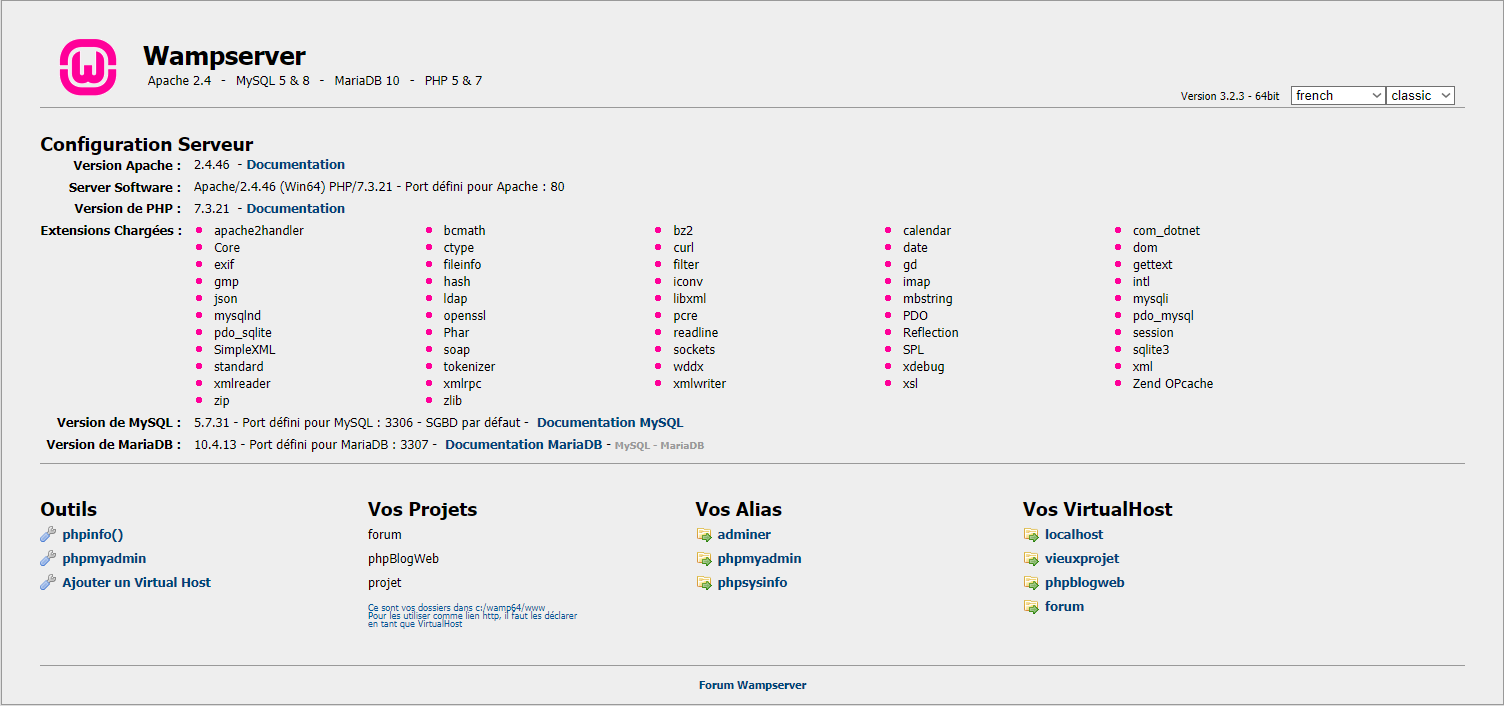
\includegraphics[width=\textwidth]{images/wamp.PNG}\\
    
    Cliquez sur "créer une virtualhost" et renseigné le chemin absolu du projet.\\
    
    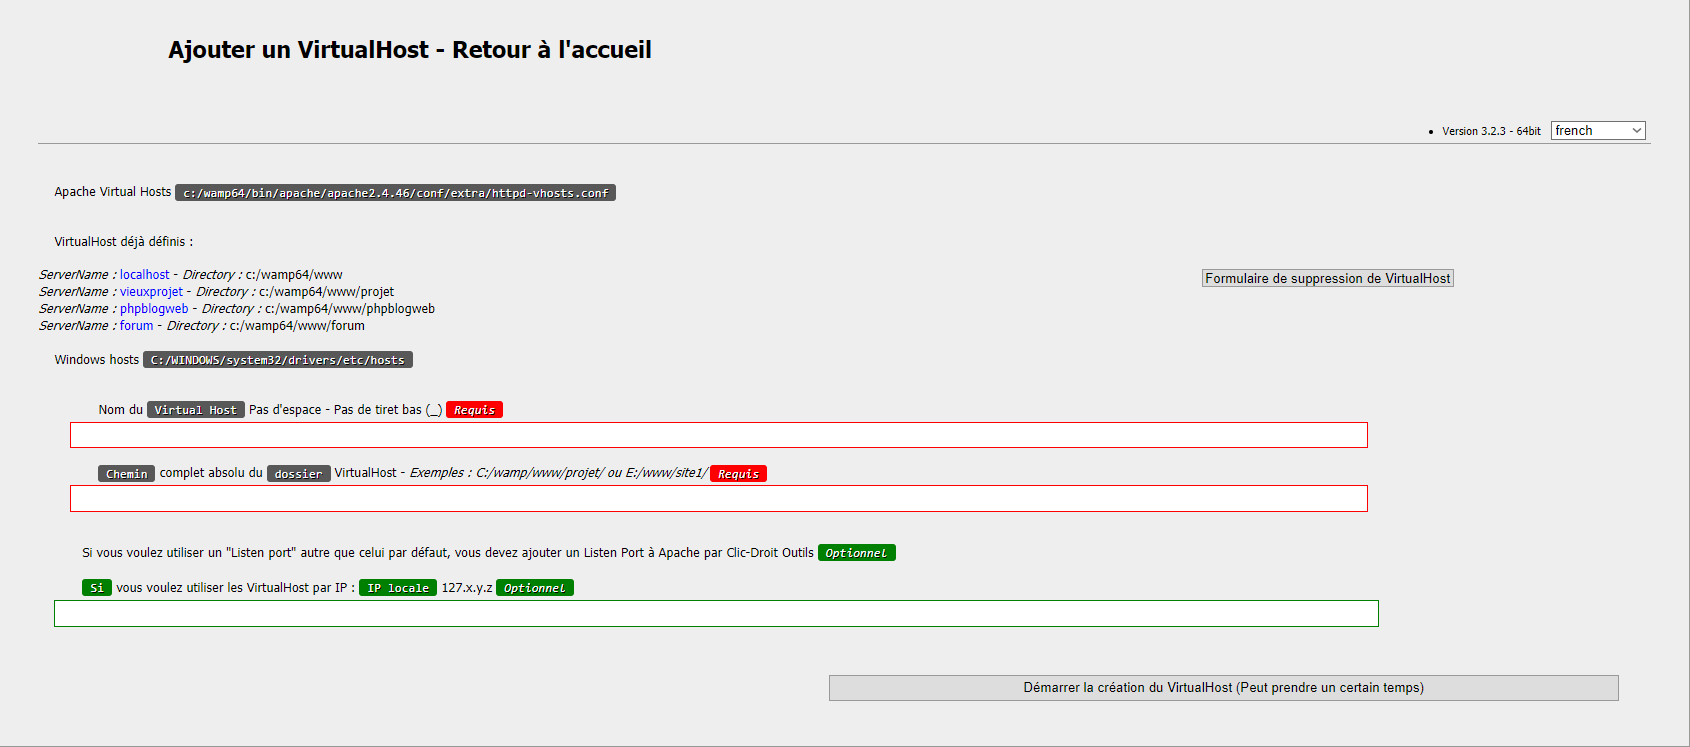
\includegraphics[width=\textwidth]{images/virtualhost.PNG}\\
    
    Il ne reste plus qu'à redémarrer 
    wamp (clique gauche sur l'icone puis "rafraichir") et de revenir sur l'accueil de Wamp. Un lien pour le projet sera présent.
    Avant de cliquer dessus, il vous faudra importer la base de donnée fournie avec le projet. Pour se faire, cliquez sur phpmyadmin
    dans la catégorie "outils" de l'accueil. Vous serez redirigé sur une page de connexion.\\


    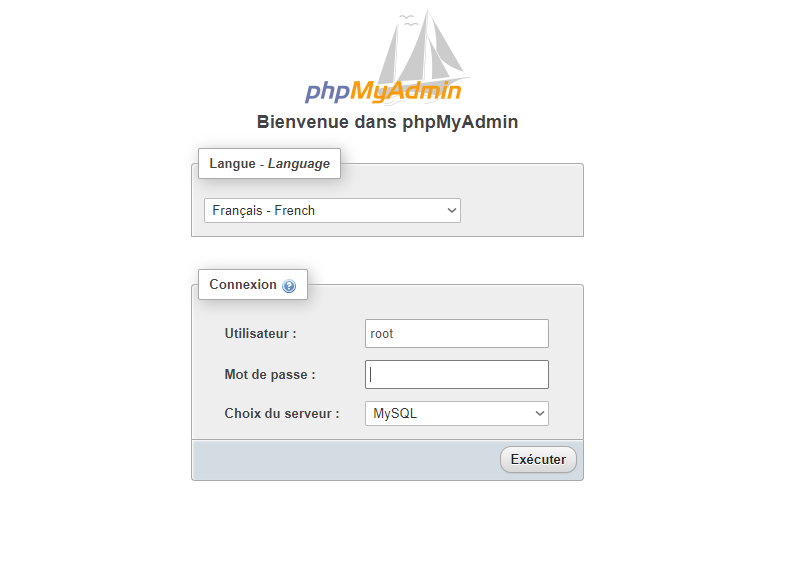
\includegraphics[width=\textwidth]{images/myadmin.PNG}\\

    L'identifiant est "root". Il n'y a pas de mot de passe (par défaut). Une fois sur phpMyAdmin, créez une base en la nommant "dbblog" puis cliquez sur "importer" et insérez le
    fichier "dbblog.sql" avant d'exécuter. Si tout se passe bien, la base de donnée devrait être opérationnelle. Le reste est pris en
    charge par notre projet.\\

    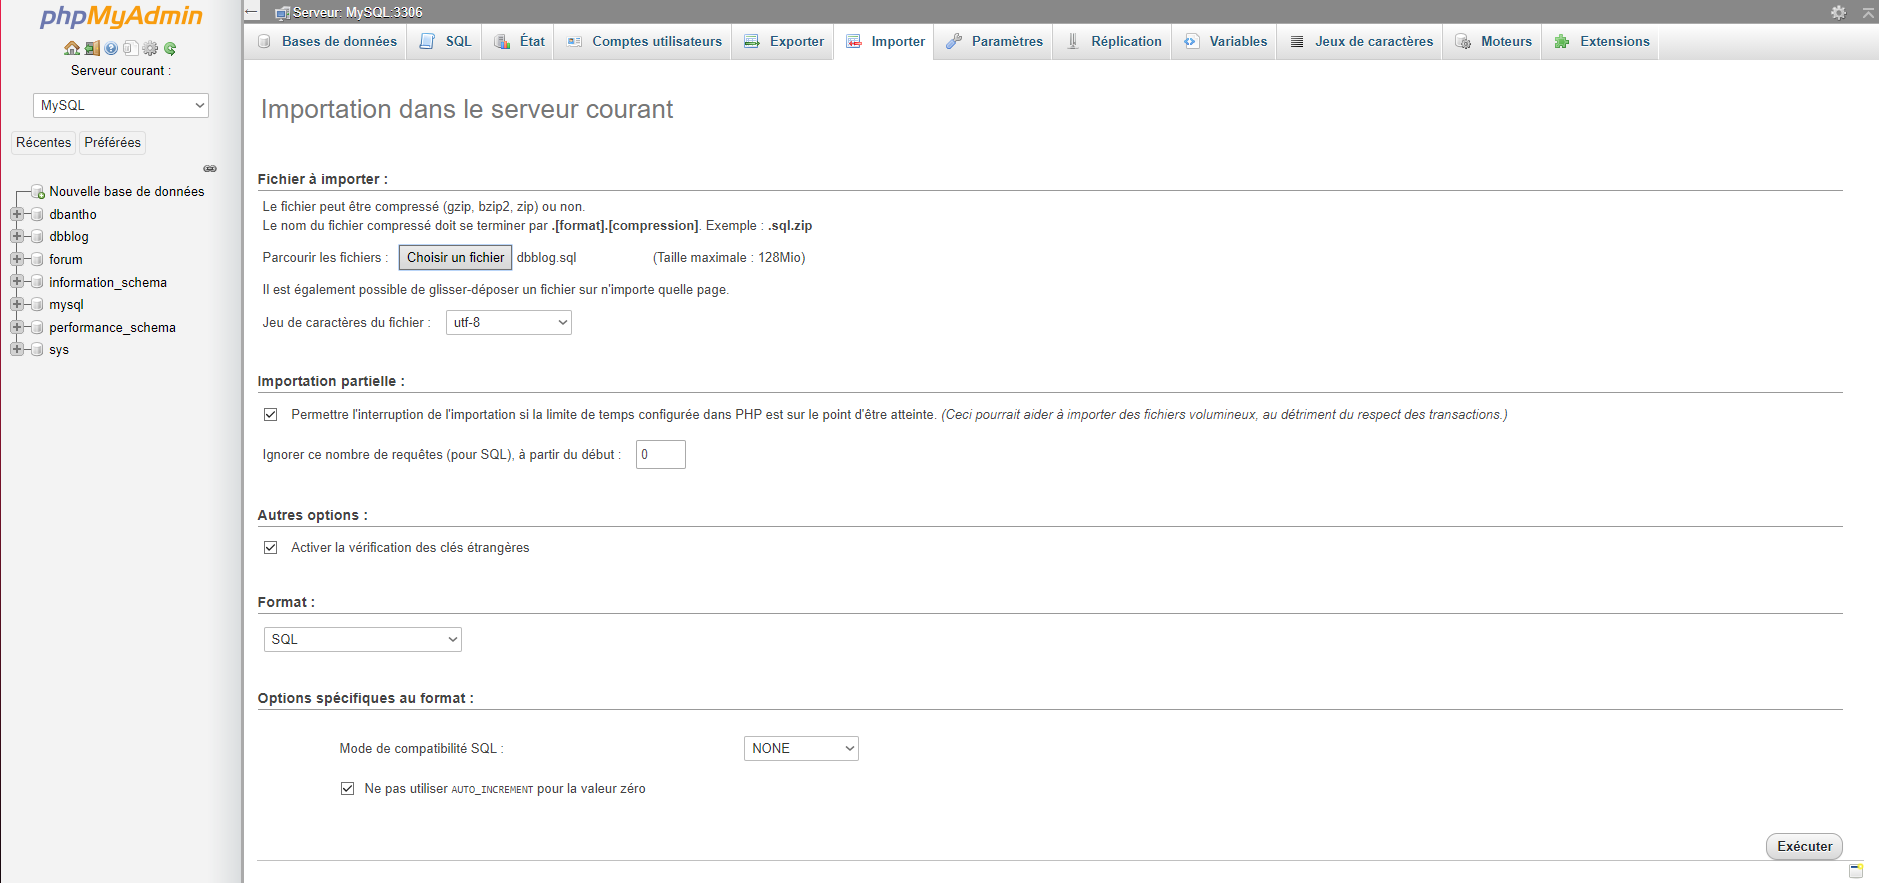
\includegraphics[width=\textwidth]{images/importbdd.PNG}\\

    \section{Problèmes rencontrés}
    Le problème principal rencontré durant ce projet était le manque d'expériences et de connaissance dans le domaine, ce qui est normal.
    Ce projet était justement là pour nous donner cette expérience. Il a fallu apprendre sur le tas en se percutant à plusieurs obstacles.
    Nous avons commis une erreur dès le début de notre projet, mais nous l'avons découverte bien trop tard : Nous avons voulu gérer toutes
    les actions de l'utilisateur avec notre variable "action" et avec des formulaires. La variables "action" nous a permis d'avoir de la
    cohérence dans notre code, ainsi qu'une certaine routine dans l'ajout de fonctionnalités. Lorsque l'utilisateur clique sur un bouton,
    la variable \$action change et suivant sa valeur, le bon contrôleur est appelé pour traiter la demande. La suite est gérée par notre
    fichier simplemodele.php.\\\\
    Nous trouvions cette approche très pratique de notre coté. Mais vers la fin du projet, nous nous sommes rendu compte des problèmes
    engendrés par cette méthode. Tout d'abord, l'utilisation abusive de formulaire en html (notamment des boutons submit) fait que lorsque
    l'utilisateur souhaite revenir en arrière en utilisant la touche "précédent" de son navigateur, ce dernier lui demandait de confirmer
    l'envoi du formulaire. Cette confirmation est très frustrante en tant qu'utilisateur. L'idée aurait été de garder les formulaires
    pour la connexion/l'inscription puis de gérer le reste sans. Mais notre variable \$action ne peut exister que dans un formulaire 
    (une balise input de type hidden pour changer la valeur de cette variable).\\
    Le deuxième problème engendré par cette méthode est que la variable \$action garde sa valeur même après le traitement de la requête.
    Pour faire simple : Quand un membre envoie un commentaire en cliquant sur "envoyer", la variable \$action prend la valeur "ajoutComm"
    ce qui permet au contrôleur CtrlMembre d'enregistrer le commentaire en base de donnée avant de rafraichir la page. Si l'utilisateur
    rafraichit la page manuellement, tout le traitement expliqué ci-dessus est ré-exécuté, dupliquant son commentaire en base de donnée.

    \section{Conclusion}
    Dans l'ensemble, nous sommes ravis d'avoir travaillé sur ce projet. Bien que le résultat final ne soit pas à la hauteur de nos espérances,
    le projet nous a confronté à de multiples obstacles que nous avons dû passer avec plus ou moins d'élégance. Les problèmes majeurs de
    notre projet nous serviront de leçon pour nos futurs projets dans le domaine du web coté serveur.
    
\end{document}